\chapter{实验结果与分析}

整个用户态协议栈系统工程量是21386行代码,其中包含移植后的Linux内核网络协议栈。启动网络应用之前,需要先在后台运行用户态协议栈进程,根据用户配置的进程个数和CPU核掩码,用户态协议栈进程以100\%的CPU占用率独占专用的CPU核。此外前端模块通过GCC编译成为动态链接SO库,接下来就可以启动网络应用服务器进程,等待客户端进行网络连接请求。在完成对整个系统的设计与开发实现后,就需要对多种主流网络应用进行移植,并且在保证不修改网络应用任何源码的前提下获得网络性能的提升。本章首先对实验环境的搭建进行简介,然后对移植后的Nginx、Lighttpd、Redis网络应用与4.15版本Linux内核的网络性能进行对比,重点关注网络延迟和吞吐。

\section{实验环境配置}
实验环境的搭建主要由三台高性能网络服务器和一台光交换机组成,实验拓扑如下图~\ref{fig:topo}所示,其中高性能网络服务器的配置均采用10Gb 82599ES Intel网卡,志强E5系列2.1Ghz主频的CPU,光交换机的配置是Mellanox公司生产的SN2100系列16端口100Gb带宽,两台服务器作为客户机与光交换机通过光纤直连,一台服务器作为运行网络应用作为服务器等待客户连接并与光交换机通过光纤直连。

\vspace{-10pt}
\begin{figure}[H] % use float package if you want it here
  \centering
  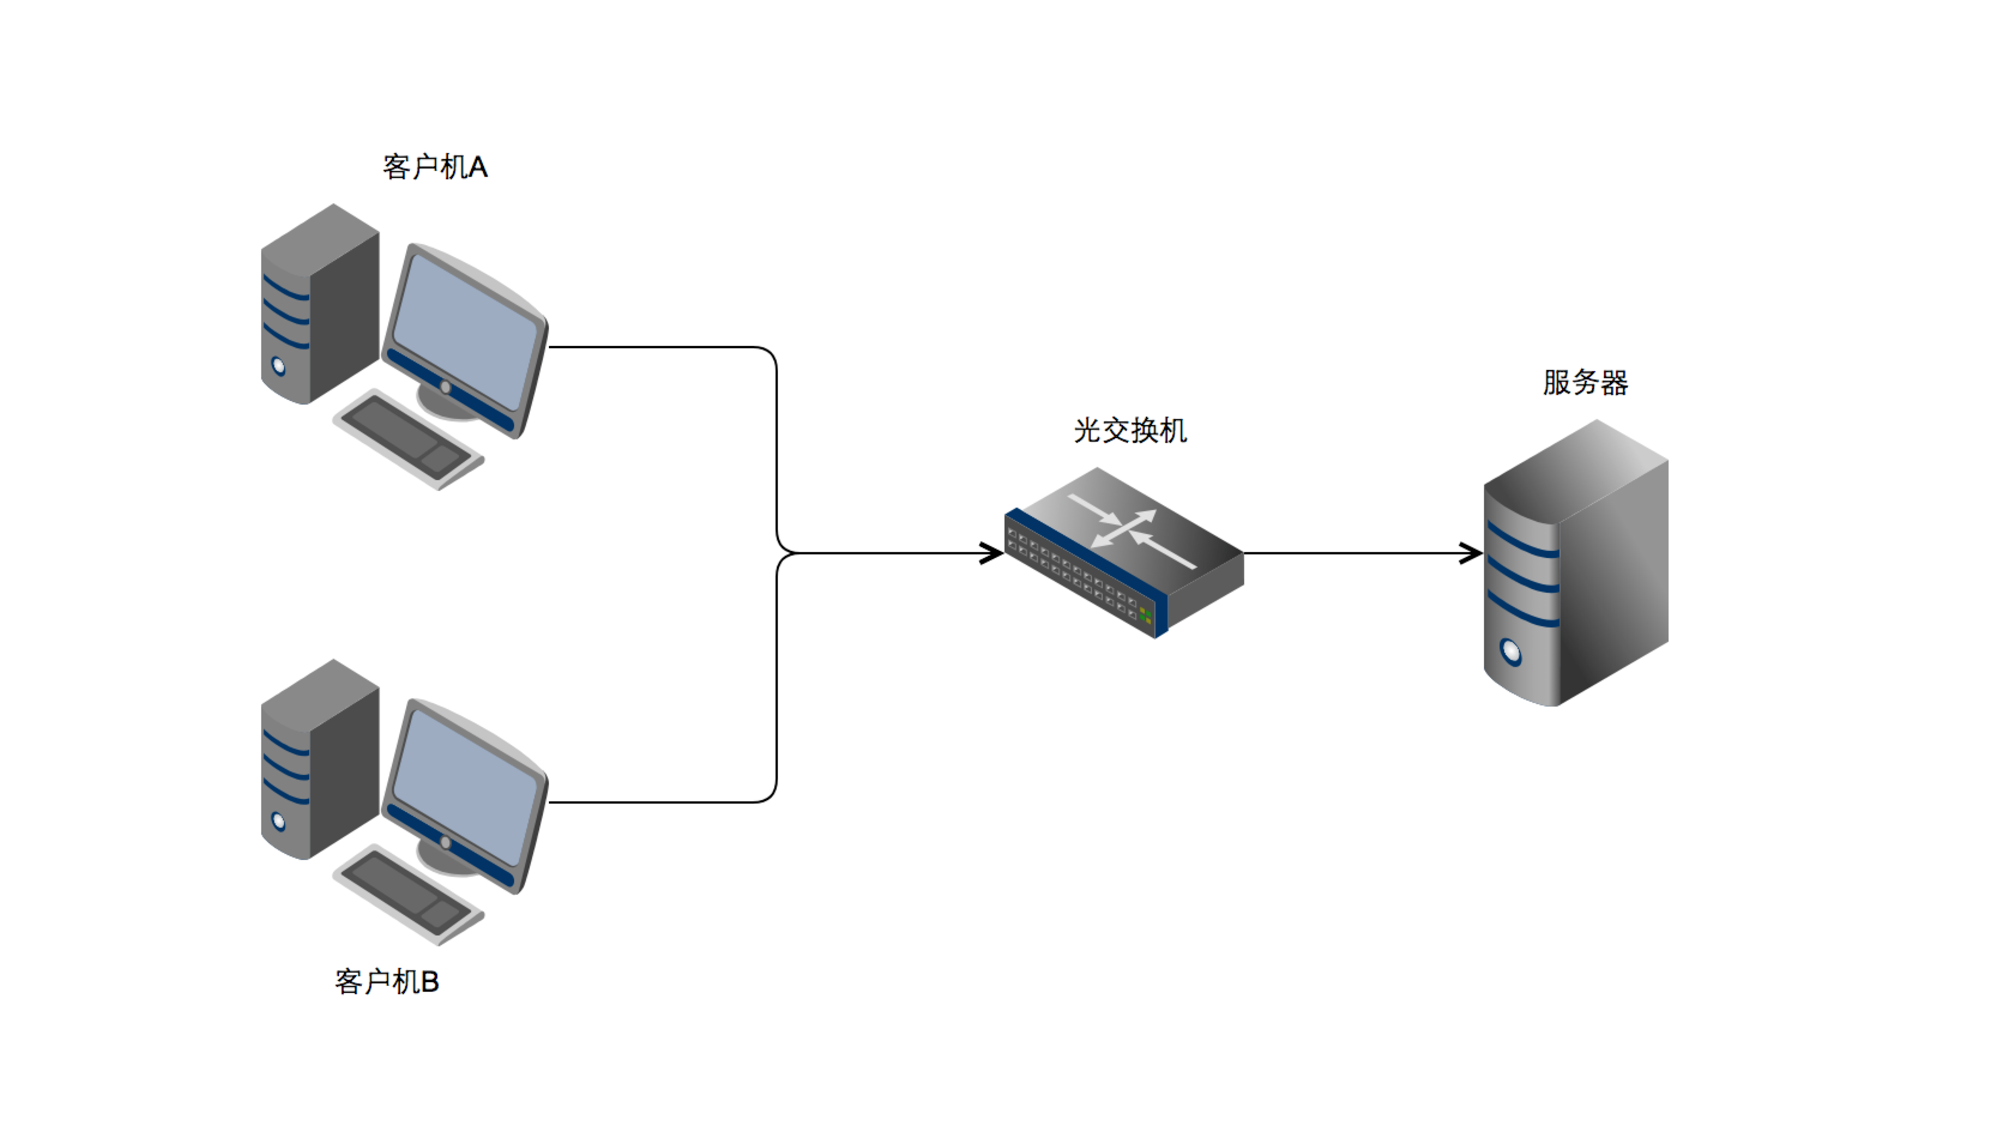
\includegraphics[width=\textwidth]{topo}
  \caption{实验环境拓扑图}
  \label{fig:topo}
\end{figure}
\vspace{-10pt}

网络应用所在服务器采用Ubuntu14.04、16.04和18.04均能完成应用的成功移植。为保证对比最新的基准,Linux使用经过零拷贝等优化的4.15内核版本,实验测试最终三台网络服务器都采用18.04版本的Ubuntu系统。实验性能本应该与同样具备应用兼容性的高性能用户态协议栈Fastsocket进行,不过按照其官网教程~\cite{fastsocket-release}进行配置后其运行性能远远低于论文中的性能,向论文作者寻求帮助后依然没有将其性能进行复现。此外,对于具备POSIX-Like API的用户态协议栈mTCP和F-stack,由于它们都移植了Lighttpd这款网络应用,所以本文为与其进行性能对比而移植Lighttpd。IX、ZygOS由于API语义完全脱离传统POSIX API并且其官方没有给出主流网络应用的移植实验成果,所以本文就未与其进行实验对比。综上所述,本章移植Nginx、Redis并与Linux 4.15版本内核网络协议栈进行性能对比,移植Lighttpd同时与Linux 4.15版本、mTCP进行性能对比。
\section{Nginx实验结果}
Nginx~\cite{Nginx}是当前最为广泛使用的Web应用服务器,既可以用来作为静态资源服务器,又可以做反向代理,利用Epoll实现在较低服务器资源消耗下达到高并发网络处理,其支持单进程运行和多进程主从运行两种模式。本用户态协议栈对两种运行模式都予以支持。在移植初期为保证Nginx服务器运行正常,通常采用两台机器直连,一台作为服务器,另一台作为客户机,在客户机使用wget进行Nginx网络连通性测试,并检测下载得到的静态文件是否正确来验证Nginx是否成功工作。

在保证Nginx运行无误后,为了模拟高并发高吞吐的网络环境,本实验在如图~\ref{fig:topo}的环境下,在两台客户机上同时使用wrk~\cite{wrk}benchmark工具,开启64个线程、512个并发连接进行1分钟的压力测试,在服务器上分别基于4.15版本Linux内核协议栈和本用户态协议栈运行1.9.5稳定版本的Nginx。由于本系统采用协议栈进程与网络应用进程分核的设计方式,即Nginx网络worker进程与用户态协议栈进程是成对出现的,所以实验使用的CPU核数是两核、四核、六核、八核、十核这五种。为了保证实验公平性,通过BIOS只开启对应的物理核,并且用户态协议栈两核(一个协议栈进程+一个Nginx worker进程)的性能是与Linux网络协议栈(两个Nginx worker)进行对比,因为二者所占用的CPU资源数是一样的。此外,实验将Nginx的keepalive时间设置为0,即一次TCP完整连接只进行一次静态文件的请求与响应,并且静态文件的大小统一设置为64B,这是为了模拟真实网络环境中的短连接。在这样的环境配置下进行实验得到如下用户态协议栈与Linux内核协议栈吞吐对比图~\ref{fig:NginxRPS}以及平均延迟对比图~\ref{fig:NginxAvg}。

\vspace{-10pt}
\begin{figure}[H] % use float package if you want it here
  \centering
  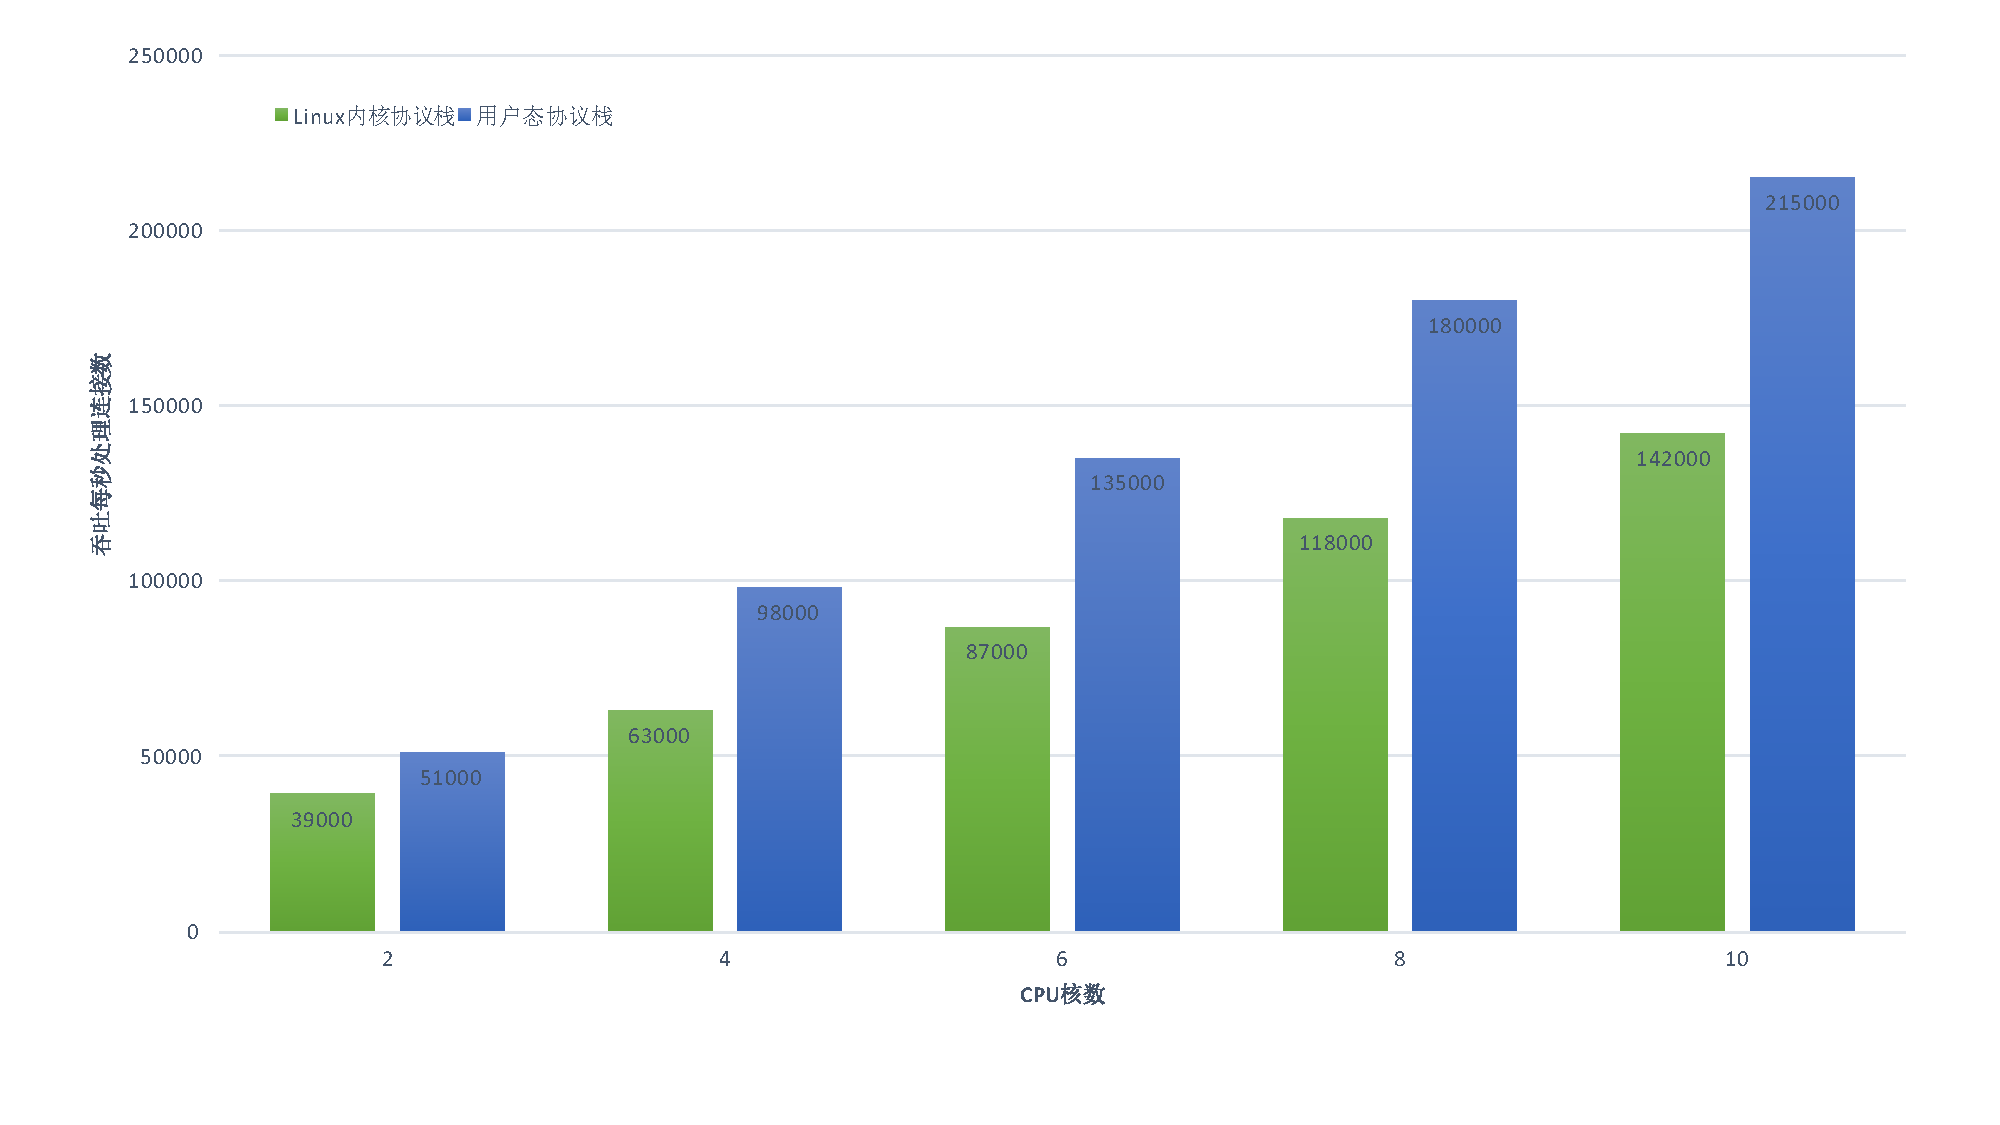
\includegraphics[width=\textwidth]{NginxRPS}
  \caption{Nginx网络吞吐性能对比图}
  \label{fig:NginxRPS}
\end{figure}
\vspace{-10pt}

\vspace{-10pt}
\begin{figure}[H] % use float package if you want it here
  \centering
  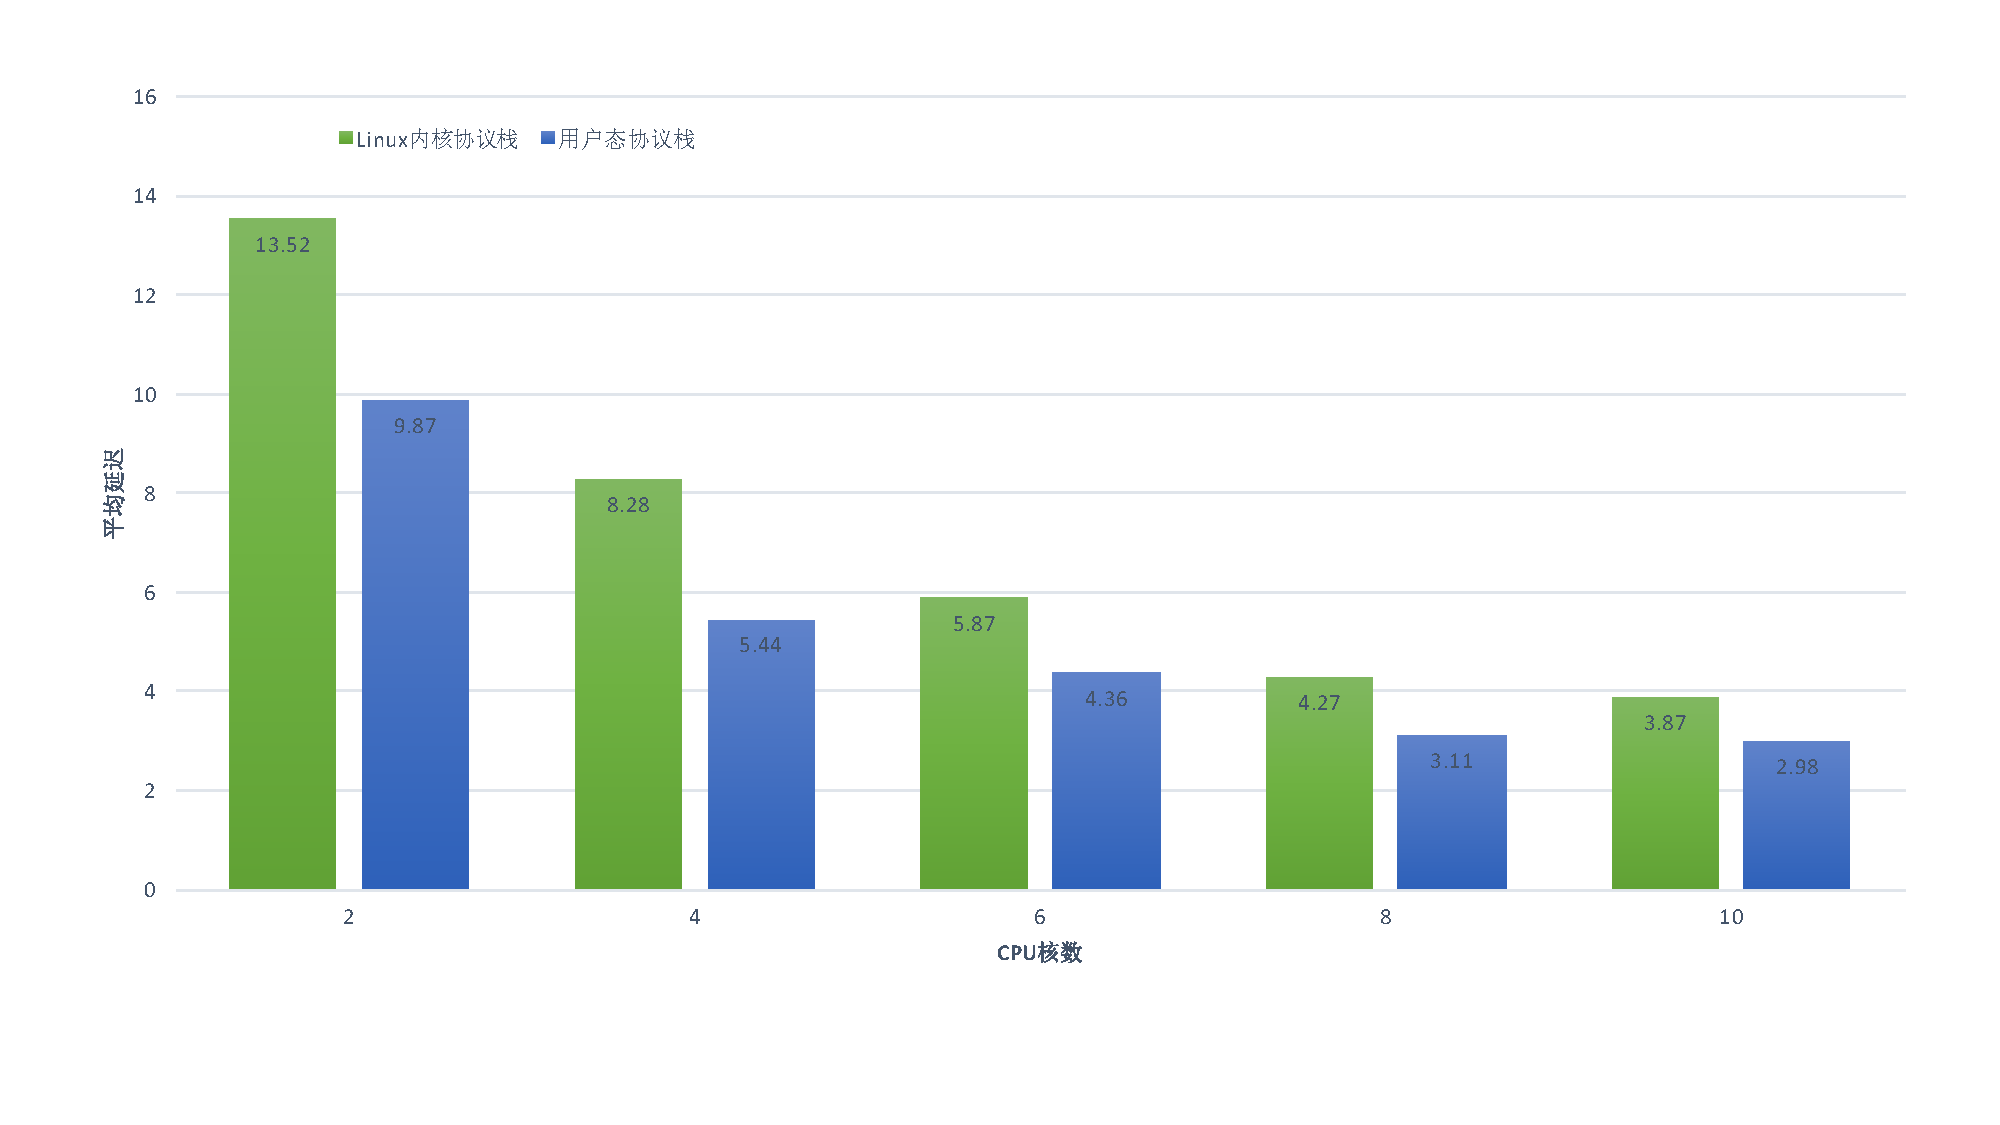
\includegraphics[width=\textwidth]{NginxAvg}
  \caption{Nginx平均延迟性能对比图}
  \label{fig:NginxAvg}
\end{figure}
\vspace{-10pt}

两图的横轴都是占用CPU的核数,纵轴分别是每秒处理连接数RPS(request per second)和平均延迟(单位是毫秒),本用户态协议栈相比Linux内核协议栈在二核、四核、六核、八核、十核下网络吞吐RPS分别提升30\%、55\%、55\%、52\%、51\%,而平均延迟分别降低27\%、34\%、25\%、27\%、22\%。网络延迟是网络服务质量中重要指标,本实验还利用wrk工具配合编写的测量延迟lua脚本,在二核的情况下对分别基于该用户态协议栈与Linux内核协议栈的Nginx网络延迟进行更加详细的统计与对比,绘制成如下延迟累积分布图~\ref{fig:NginxTail},横轴是延迟,单位是毫秒。可以看到,在99.9999\%对应的用户态协议栈延迟是24.98ms,相比内核协议栈268.5ms降低了90\%之多。尾延迟的大幅降低对于网络游戏这类延迟敏感性要求高的网络应用有着重要意义。

\vspace{-10pt}
\begin{figure}[H] % use float package if you want it here
  \centering
  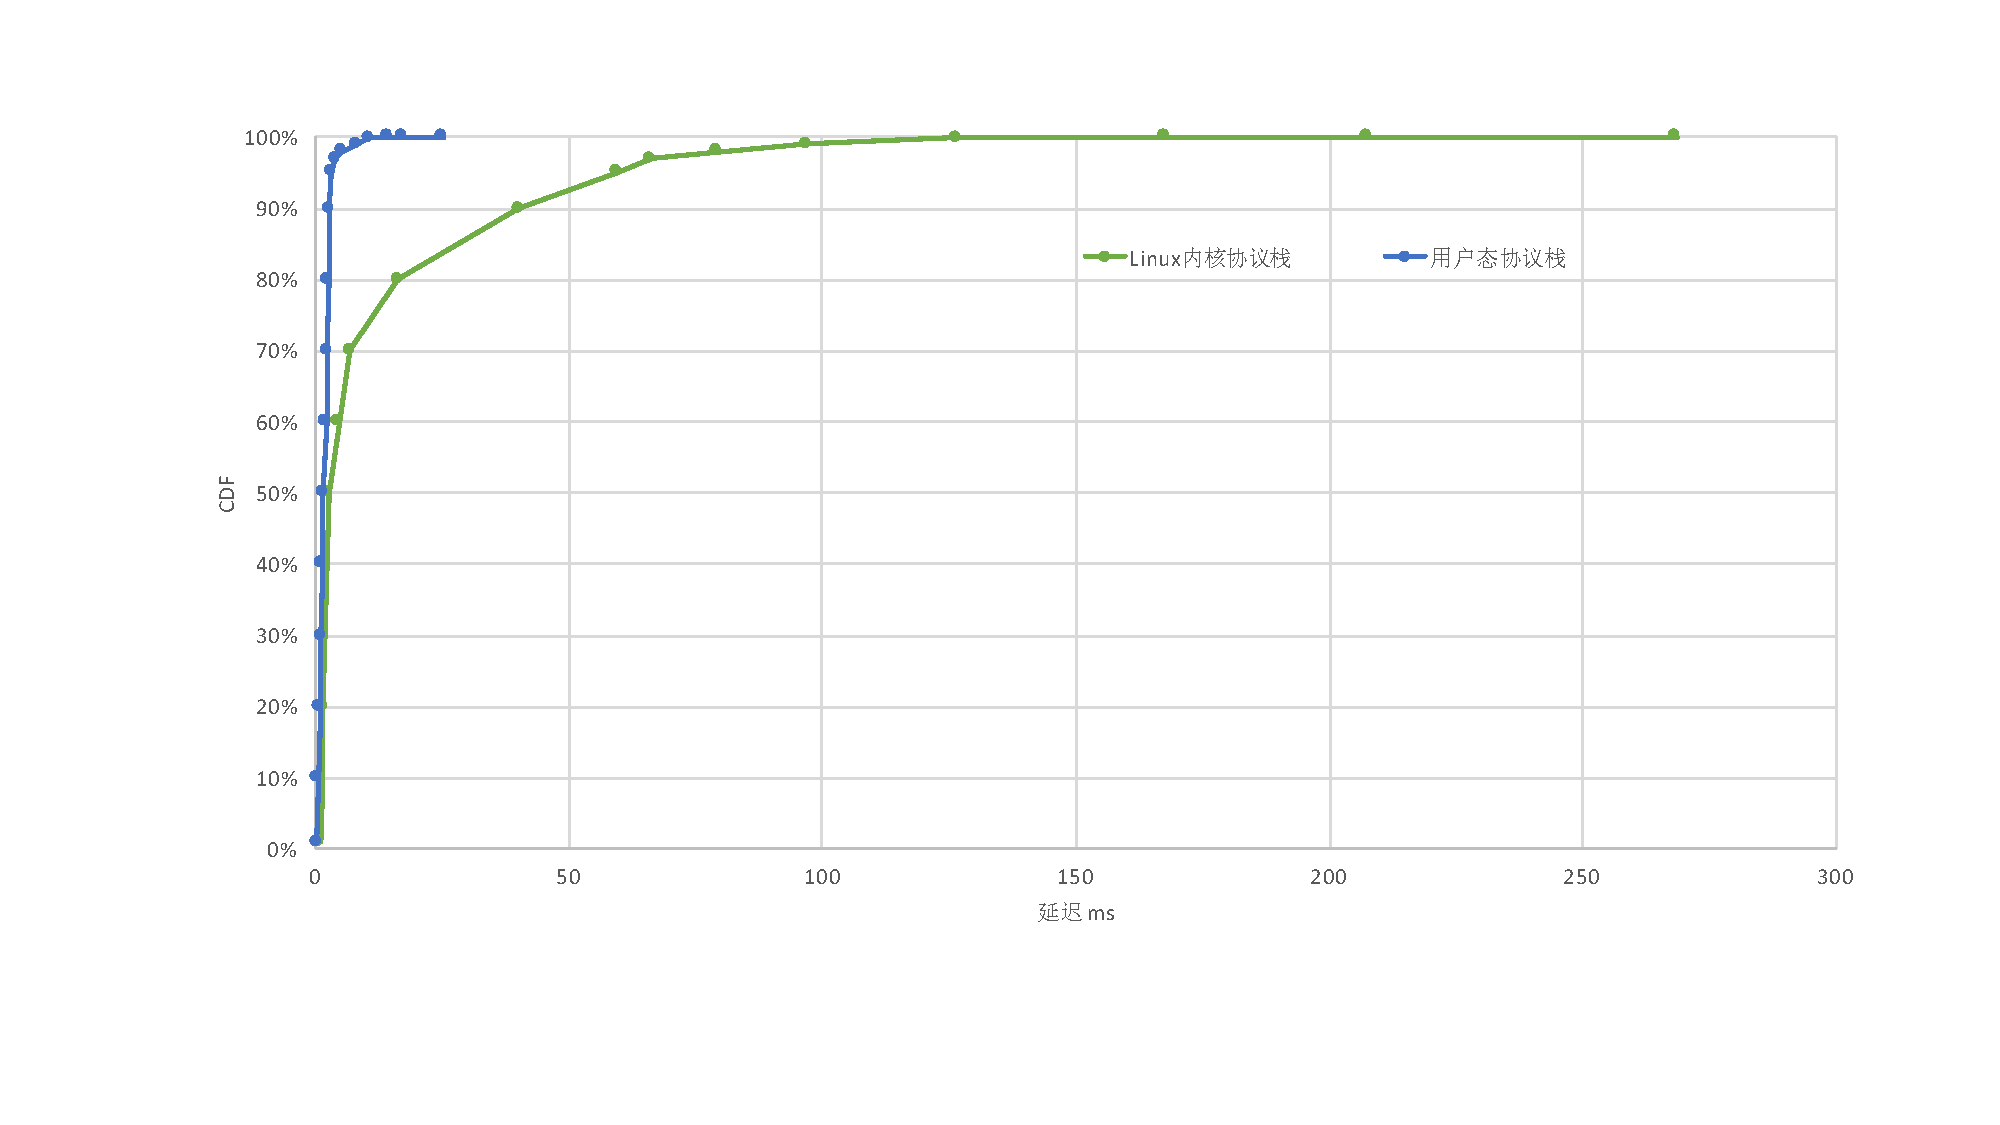
\includegraphics[width=\textwidth]{NginxTail}
  \caption{Nginx延迟累积分布图}
  \label{fig:NginxTail}
\end{figure}
\vspace{-10pt}

\section{Lighttpd实验结果}
Lighttpd相比Nginx、Apache是一个更加轻量级的Web服务器,其工作模式与Nginx类似,支持单进程模式和多进程主从模式。目前业界影响力最大并且开源的用户态协议栈mTCP已成功移植Lighttpd,为了与mTCP进行性能对比,本文将Lighttpd移植到本用户态协议栈上,移植过程中遇到的两点问题已经成功解决,第一个问题是返回给Lighttpd应用的套接字文件描述符过大从而导致数组越界访问,第二个问题是Lighttpd不像Nginx可以在配置文件中对worker进程设置亲核性,这导致Lighttpd的worker进程与协议栈进程发生严重的CPU资源争抢,这两个问题已经在兼容性设计一节中详细描述,此处不予赘述。实验依然使用wrk这款benchmark工具进行压力测试,两个客户机同时开启64个线程,512个并发连接对服务器进行压力测试,得到在双核下与Linux内核协议栈、mTCP的性能对比图如下~\ref{fig:compare},相比Linux内核协议栈性能提升37\%,不过由于本用户态协议栈运行一个worker需要占用两个核,与mTCP对比时候是其运行两个mTCP线程与两个网络应用线程,这样相比之下本用户态协议栈的性能确实只有mTCP的66\%。当然mTCP移植网络应用需要对其所有网络POSIX API进行修改,而本用户态协议栈可以在完全不需要修改任何源码的前提下为传统网络应用带来性能提升,除此之外mTCP只是简易TCP/IP协议栈,不具备UDP功能以及抵御网络安全攻击的能力较差,这也是本协议栈相比mTCP的优势。

\vspace{-10pt}
\begin{figure}[H] % use float package if you want it here
  \centering
  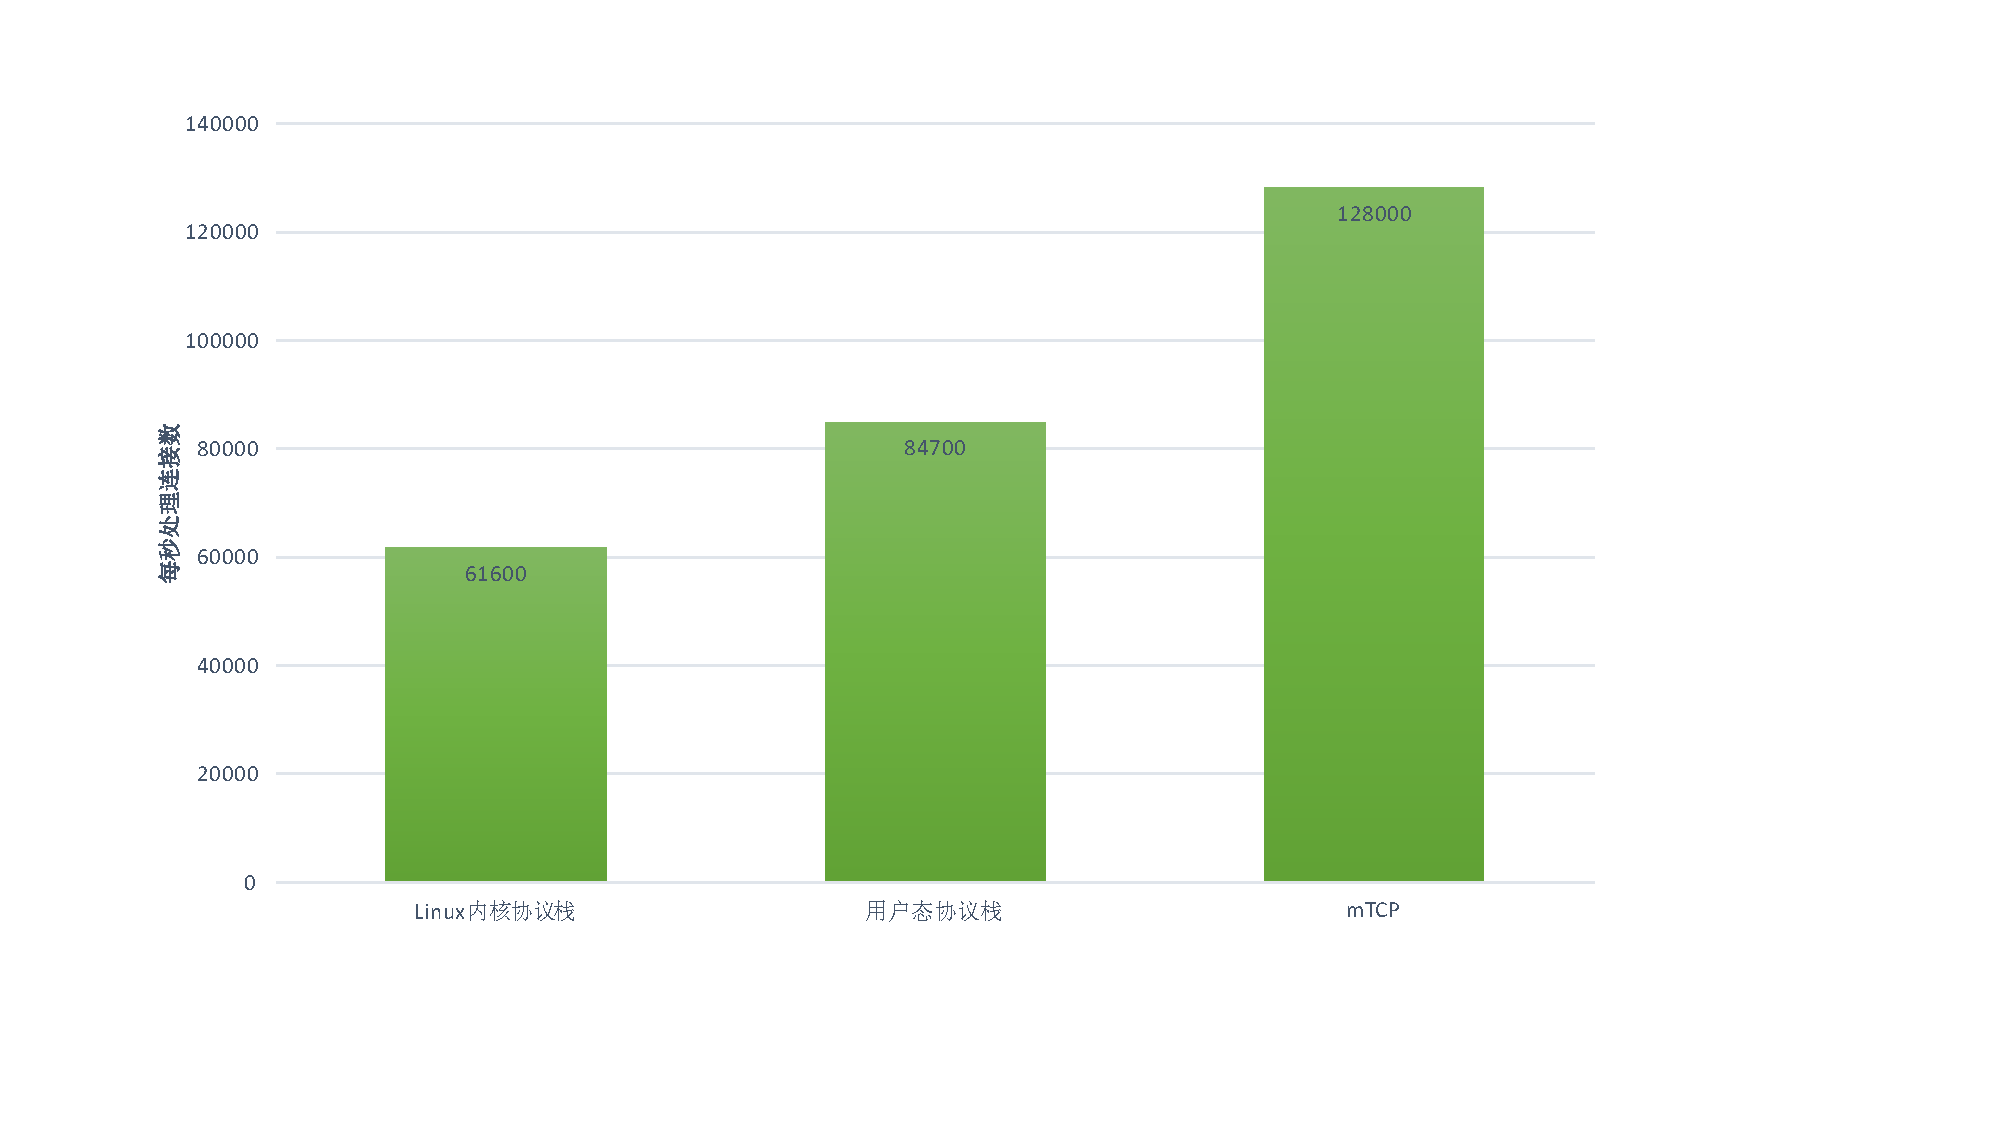
\includegraphics[width=\textwidth]{compare}
  \caption{Lighttpd性能对比图}
  \label{fig:compare}
\end{figure}
\vspace{-10pt}

\vspace{-10pt}
\begin{figure}[H] % use float package if you want it here
  \centering
  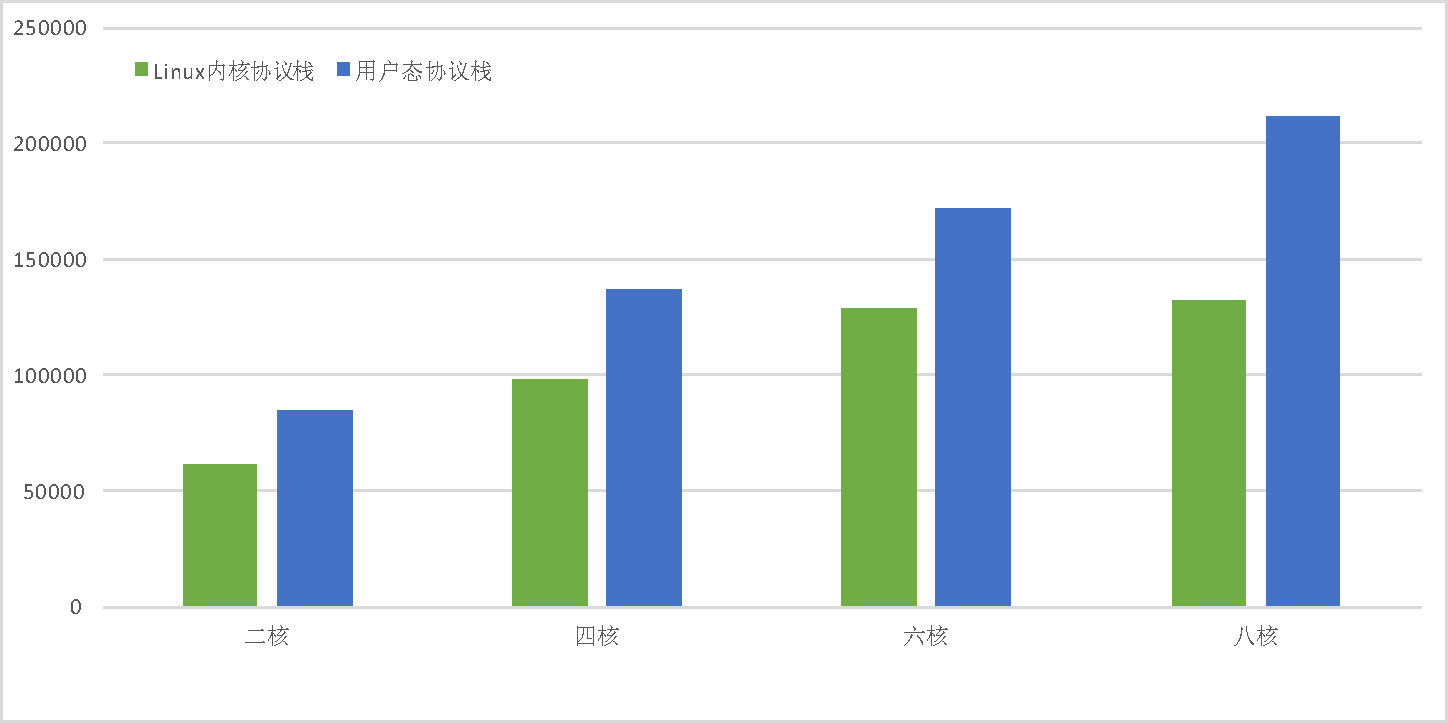
\includegraphics[width=\textwidth]{LighttpdRPS}
  \caption{Lighttpd多核性能对比图}
  \label{fig:LighttpdRPS}
\end{figure}
\vspace{-10pt}

与此同时也对Lighttpd移植后的多核吞吐性能进行实验,与Nginx实验方式一样在二核、四核、六核、八核下进行压力测试,得到如图~\ref{fig:LighttpdRPS}的多核吞吐网络性能对比图。

\section{Redis实验结果}

在内存计算领域,Key Value存储已成为分布式系统中存储共享数据结构的重要基础设施服务。在生产环境中,许多数据结构可以用一个键值哈希表来表示,例如在NoSQL数据库中的数据索引、机器学习训练中的模型参数、图形计算中的节点和边缘以及分布式同步中的序列器,这使得Redis、Memcached等Key Value内存服务器被广泛使用。当前物理内存与网卡控制器的带宽资源已经不在成为系统的性能瓶颈,内核网络协议栈就成为KV存储服务器在高并发网络环境下的性能短板。所以,本工作将Redis这款目前业界最为常用的KV内存服务器移植到该用户态协议栈上。由于Redis只有单进程一种工作模式,而如果要进行横向扩展则通常使用分布式的策略,所以本实验仅使用两个物理核对Redis基于本用户态协议栈和Linux内核协议栈进行对比,服务器端运行Redis Server进程,而在客户机中运行Redis自带的benchmark工具并在100个网络并发下进行100w次不同命令的压力测试,在此仅列举出GET、PUT两种较为常见的内存KV操作。

\vspace{-10pt}
\begin{figure}[H] % use float package if you want it here
  \centering
  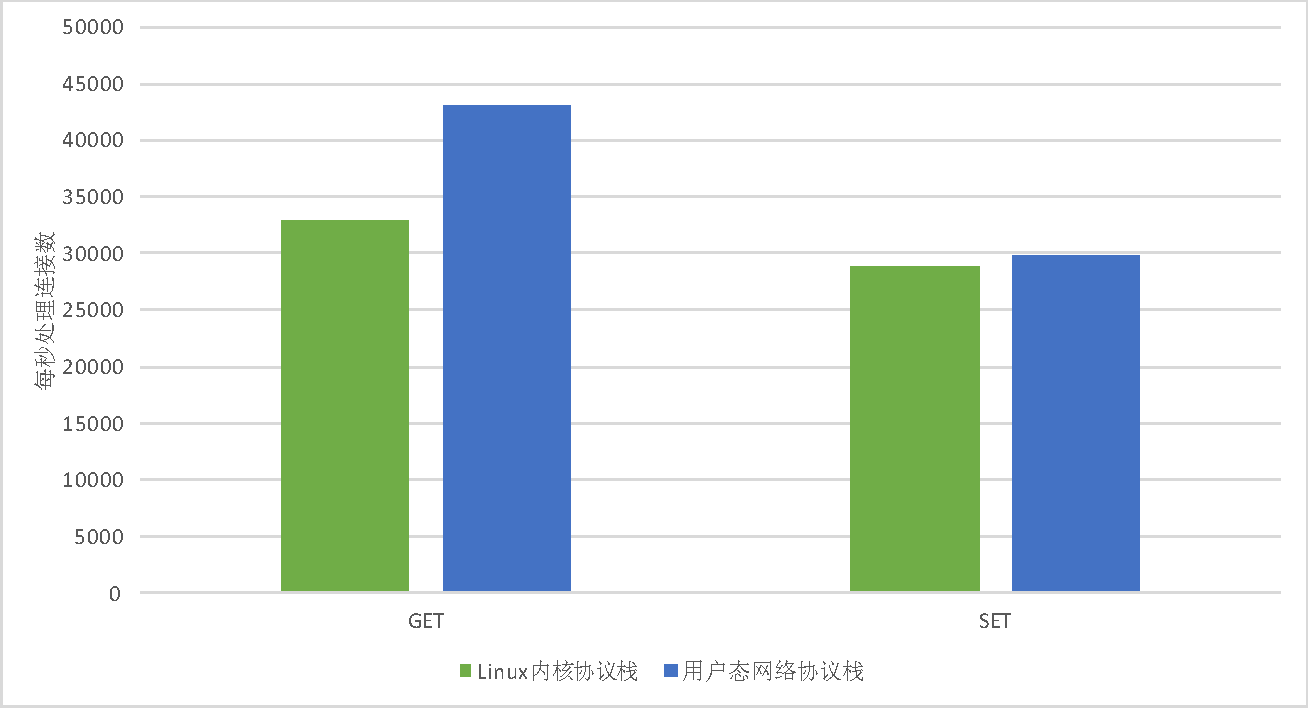
\includegraphics[width=\textwidth]{redisRPS}
  \caption{Redis性能对比图}
  \label{fig:redisRPS}
\end{figure}
\vspace{-10pt}

性能对比如~\ref{fig:redisRPS}图所示,纵轴是每秒处理连接数,可以看到用户协议栈对于GET操作有31\%较为明显的性能提升,但对于PUT等其他操作提升有限,不过KV内存服务器中众多场景的网络流量大多由GET操作构成,这种性能提升对于真实生产环境同样具有重要意义。

\section{实验结果总结与分析}

本章对已经成功移植的Nginx、Lighttpd、Redis这三款网络应用进行压力测试与性能对比分析,可以看出本用户态协议栈系统既可以达到不需要修改传统网络应用源码的高度兼容性,同时又能为传统网络应用带来较为明显的性能提升。在Nginx、Lighttpd这类Web服务器中为每秒处理连接数带来超过50\%的性能提升,并在十核之内维持着0.88的线性扩展系数。对Redis这类Key Value内存服务器的GET操作带来超过30\%的性能提升。此外,该用户态协议栈系统还移植到自行开发的传统多进程fork网络模型与基于epoll的多线程网络模型等多种网络服务器,均获得超过40\%的性能提升。